%%%%%%%%%%%%%%%%%%%%%%%%%%%%%%%%%%%%%%%%%%%%%%%%%%%%%%%%%%%%%%%
%% BRIEF VERSION OF OXFORD THESIS TEMPLATE FOR CHAPTER PREVIEWS

%%%%% CHOOSE PAGE LAYOUT
% format for PDF output (ie equal margins, no extra blank pages):
\documentclass[a4paper,nobind]{templates/ociamthesis}

% UL 5 January 2021 - add packages used by kableExtra
\usepackage{booktabs}
\usepackage{longtable}
\usepackage{array}
\usepackage{multirow}
\usepackage{wrapfig}
\usepackage{colortbl}
\usepackage{pdflscape}
\usepackage{tabu}
\usepackage{threeparttable}
\usepackage{threeparttablex}
\usepackage[normalem]{ulem}
\usepackage{makecell}
\usepackage[colorlinks=false,pdfpagelabels,hidelinks=]{hyperref}
\usepackage{float}


%UL set section header spacing
\usepackage{titlesec}
% 
\titlespacing\subsubsection{0pt}{24pt plus 4pt minus 2pt}{0pt plus 2pt minus 2pt}

% UL 30 Nov 2018 pandoc puts lists in 'tightlist' command when no space between bullet points in Rmd file
\providecommand{\tightlist}{%
  \setlength{\itemsep}{0pt}\setlength{\parskip}{0pt}}
 
% UL 1 Dec 2018, fix to include code in shaded environments
\usepackage{color}
\usepackage{fancyvrb}
\newcommand{\VerbBar}{|}
\newcommand{\VERB}{\Verb[commandchars=\\\{\}]}
\DefineVerbatimEnvironment{Highlighting}{Verbatim}{commandchars=\\\{\}}
% Add ',fontsize=\small' for more characters per line
\usepackage{framed}
\definecolor{shadecolor}{RGB}{248,248,248}
\newenvironment{Shaded}{\begin{snugshade}}{\end{snugshade}}
\newcommand{\AlertTok}[1]{\textcolor[rgb]{0.94,0.16,0.16}{#1}}
\newcommand{\AnnotationTok}[1]{\textcolor[rgb]{0.56,0.35,0.01}{\textbf{\textit{#1}}}}
\newcommand{\AttributeTok}[1]{\textcolor[rgb]{0.77,0.63,0.00}{#1}}
\newcommand{\BaseNTok}[1]{\textcolor[rgb]{0.00,0.00,0.81}{#1}}
\newcommand{\BuiltInTok}[1]{#1}
\newcommand{\CharTok}[1]{\textcolor[rgb]{0.31,0.60,0.02}{#1}}
\newcommand{\CommentTok}[1]{\textcolor[rgb]{0.56,0.35,0.01}{\textit{#1}}}
\newcommand{\CommentVarTok}[1]{\textcolor[rgb]{0.56,0.35,0.01}{\textbf{\textit{#1}}}}
\newcommand{\ConstantTok}[1]{\textcolor[rgb]{0.00,0.00,0.00}{#1}}
\newcommand{\ControlFlowTok}[1]{\textcolor[rgb]{0.13,0.29,0.53}{\textbf{#1}}}
\newcommand{\DataTypeTok}[1]{\textcolor[rgb]{0.13,0.29,0.53}{#1}}
\newcommand{\DecValTok}[1]{\textcolor[rgb]{0.00,0.00,0.81}{#1}}
\newcommand{\DocumentationTok}[1]{\textcolor[rgb]{0.56,0.35,0.01}{\textbf{\textit{#1}}}}
\newcommand{\ErrorTok}[1]{\textcolor[rgb]{0.64,0.00,0.00}{\textbf{#1}}}
\newcommand{\ExtensionTok}[1]{#1}
\newcommand{\FloatTok}[1]{\textcolor[rgb]{0.00,0.00,0.81}{#1}}
\newcommand{\FunctionTok}[1]{\textcolor[rgb]{0.00,0.00,0.00}{#1}}
\newcommand{\ImportTok}[1]{#1}
\newcommand{\InformationTok}[1]{\textcolor[rgb]{0.56,0.35,0.01}{\textbf{\textit{#1}}}}
\newcommand{\KeywordTok}[1]{\textcolor[rgb]{0.13,0.29,0.53}{\textbf{#1}}}
\newcommand{\NormalTok}[1]{#1}
\newcommand{\OperatorTok}[1]{\textcolor[rgb]{0.81,0.36,0.00}{\textbf{#1}}}
\newcommand{\OtherTok}[1]{\textcolor[rgb]{0.56,0.35,0.01}{#1}}
\newcommand{\PreprocessorTok}[1]{\textcolor[rgb]{0.56,0.35,0.01}{\textit{#1}}}
\newcommand{\RegionMarkerTok}[1]{#1}
\newcommand{\SpecialCharTok}[1]{\textcolor[rgb]{0.00,0.00,0.00}{#1}}
\newcommand{\SpecialStringTok}[1]{\textcolor[rgb]{0.31,0.60,0.02}{#1}}
\newcommand{\StringTok}[1]{\textcolor[rgb]{0.31,0.60,0.02}{#1}}
\newcommand{\VariableTok}[1]{\textcolor[rgb]{0.00,0.00,0.00}{#1}}
\newcommand{\VerbatimStringTok}[1]{\textcolor[rgb]{0.31,0.60,0.02}{#1}}
\newcommand{\WarningTok}[1]{\textcolor[rgb]{0.56,0.35,0.01}{\textbf{\textit{#1}}}}

%UL 2 Dec 2018 add a bit of white space before and after code blocks
\renewenvironment{Shaded}
{
  \vspace{10pt}%
  \begin{snugshade}%
}{%
  \end{snugshade}%
  \vspace{8pt}%
}
%UL 2 Dec 2018 reduce whitespace around verbatim environments
\usepackage{etoolbox}
\makeatletter
\preto{\@verbatim}{\topsep=0pt \partopsep=0pt }
\makeatother

%UL 28 Mar 2019, enable strikethrough
\usepackage[normalem]{ulem}

%UL use soul package for correction highlighting
\usepackage{soul}
\usepackage{xcolor}
\newcommand{\ctext}[3][RGB]{%
  \begingroup
  \definecolor{hlcolor}{#1}{#2}\sethlcolor{hlcolor}%
  \hl{#3}%
  \endgroup
}
\soulregister\ref7
\soulregister\cite7
\soulregister\autocite7
\soulregister\textcite7
\soulregister\pageref7

%UL 3 Nov 2019, avoid mysterious error from not having hyperref included
\usepackage{hyperref}

%%%%% SELECT YOUR DRAFT OPTIONS
% Three options going on here; use in any combination.  But remember to turn the first two off before
% generating a PDF to send to the printer!

% This adds a "DRAFT" footer to every normal page.  (The first page of each chapter is not a "normal" page.)

% This highlights (in blue) corrections marked with (for words) \mccorrect{blah} or (for whole
% paragraphs) \begin{mccorrection} . . . \end{mccorrection}.  This can be useful for sending a PDF of
% your corrected thesis to your examiners for review.  Turn it off, and the blue disappears.

%%%%% BIBLIOGRAPHY SETUP
% Note that your bibliography will require some tweaking depending on your department, preferred format, etc.
% The options included below are just very basic "sciencey" and "humanitiesey" options to get started.
% If you've not used LaTeX before, I recommend reading a little about biblatex/biber and getting started with it.
% If you're already a LaTeX pro and are used to natbib or something, modify as necessary.
% Either way, you'll have to choose and configure an appropriate bibliography format...

% The science-type option: numerical in-text citation with references in order of appearance.
% \usepackage[style=numeric-comp, sorting=none, backend=biber, doi=false, isbn=false]{biblatex}
% \newcommand*{\bibtitle}{References}

% The humanities-type option: author-year in-text citation with an alphabetical works cited.
% \usepackage[style=authoryear, sorting=nyt, backend=biber, maxcitenames=2, useprefix, doi=false, isbn=false]{biblatex}
% \newcommand*{\bibtitle}{Works Cited}

%UL 3 Dec 2018: set this from YAML in index.Rmd
\usepackage[style=numeric-comp, sorting=none, backend=biber, doi=false, isbn=false]{biblatex}
\newcommand*{\bibtitle}{References}

% This makes the bibliography left-aligned (not 'justified') and slightly smaller font.
\renewcommand*{\bibfont}{\raggedright\small}

% Change this to the name of your .bib file (usually exported from a citation manager like Zotero or EndNote).
\addbibresource{references.bib}

%%%%% YOUR OWN PERSONAL MACROS
% This is a good place to dump your own LaTeX macros as they come up.

% To make text superscripts shortcuts
	\renewcommand{\th}{\textsuperscript{th}} % ex: I won 4\th place
	\newcommand{\nd}{\textsuperscript{nd}}
	\renewcommand{\st}{\textsuperscript{st}}
	\newcommand{\rd}{\textsuperscript{rd}}

%%%%% THE ACTUAL DOCUMENT STARTS HERE
\begin{document}

%%%%% CHOOSE YOUR LINE SPACING HERE
% This is the official option.  Use it for your submission copy and library copy:
\setlength{\textbaselineskip}{22pt plus2pt}
% This is closer spacing (about 1.5-spaced) that you might prefer for your personal copies:
%\setlength{\textbaselineskip}{18pt plus2pt minus1pt}

% UL: You can set the general paragraph spacing here - I've set it to 2pt (was 0) so
% it's less claustrophobic
\setlength{\parskip}{2pt plus 1pt}

% Leave this line alone; it gets things started for the real document.
\setlength{\baselineskip}{\textbaselineskip}

% all your chapters and appendices will appear here
\begin{savequote}
``Asking for investors to come is the wrong direction completely.
\ldots{} If you are inviting investment from the market, they are
looking for their return. That is the wrong message. Micro-credit should
not be presented to investors as a ground for making a lot of money out
of the poor people -- that is a shame.''
\end{savequote}



\hypertarget{rmd-basics}{%
\chapter{Introduction}\label{rmd-basics}}

\minitoc 

\hypertarget{background-to-the-study}{%
\section{Background to the Study}\label{background-to-the-study}}

\noindent Advocates of Microfinance institutions (MFIs) hail the industry for availing financial services to the poor and the financially excluded. Data from 2015, for example, shows that MFIs availed \$92.4 billion to 116.6 million borrowers and accepted \$58.9 billion from 98.4 million depositors \autocite{market2014global}. Supporters of Microfinance (MF) further associate it with improved household welfare \autocite{meador2017food,you2013role}, increased purchasing power and a higher employment rate \autocite{raihan2017macro,lopatta2016microfinance}. Also, MF supporters contend that it leads to improved gender parity \autocite{mafukata2017reciprocal,zhang2017microfinance}, and enables families to cope with the effects of climate change \autocite{fenton2017role} among other benefits \footnote{The quotation comes from an interview of Professor Muhammad Yunus. The video is available at \url{https://nextbillion.net/an-interview-with-muhammad-yunus/}}.

Other researchers, however, have uncovered mixed outcomes from Microfinance (MF) interventions. For example, \textcite{ganle2015microcredit} found that while some women indeed get empowered as a result of access to credit, most have little control over the subsequent spending while a significant proportion suffers harassment from MF agents' for failing to repay the loans. \textcite{van2012impact} also arrive at a similar conclusion.

On the other extreme, some scholars dispute the benefits of MF altogether. For instance, some researchers posit that MF does not boost employment and education among the rural poor \autocite{bauchet2013micro}. Other researchers link micro-credit to increased child labour \autocite{hazarika2008household}, increased gender inequalities in access to finance \autocite{zulfiqar2017does}, and reduced entrepreneurial spirit among the poor \autocite{field2013does}. The apprehension around the high-interest rates charged by MFIs and inappropriate lending practices that fail to account for the social, cultural, and economic context of the target clients is also gaining prominence \autocite{chester2016one}. Taken together, the case against MF paints a bleak future of MF. Some studies recommend a re-examination of the MF business model and call for better regulation of the industry \autocite{johnson2013microfinance,ghosh2013microfinance}. Without reforms, conclude \textcite{chester2016one}, ``the MF industry could not only ruin the lives of many borrowers but also ruin itself.''

Despite these contradicting views, MFIs continue to attract interest from governments, state agencies, donor organisations, philanthropists and increasingly commercial providers of capital. Initially, MFIs ran on the non-governmental organisation (NGO) model relying chiefly on donors to finance their operations \autocite{d2017ngos}. The NGO oriented model has been emphasising the social mission of MFIs- that is, availing financial services to the poor and the financially excluded \autocite{ashta2012compartamos}. The model played down the profit motive \texttt{(ashta,\ 2013)}.

However, in the last two decades, some MFIs have been transforming their institutional structure from NGOs to commercial entities \autocite{d2017ngos}. This study seeks to evaluate the possible impacts of the transformation of MFIs on their financial sustainability and outreach to the financially excluded. Transformation is a process where an MFI converts from a donor-funded NGO to a regulated financial institution (RFI) that derives its capital primarily from commercial sources. The rationale for the transformation is that it would not only enable MFIs to access commercial sources of capital but also lead to improved financial sustainability, efficiency and social performance \autocite{louis2013financial}.

Other benefits of the transformation include improved customer service, a more extensive range of products, and enhanced control and governance\autocite{srnec2008transformation}. Consumers and other stakeholders would also reap the benefits of the regulation of MFIs both directly \textcite{meagher2006microfinance}, and indirectly \autocite{hartarska2007regulated}. Nevertheless, the process of transformation is complicated and dependent on the country-specific regulatory framework. Thus, although most research delineates a point in time when an MFI ceases to be an NGO and becomes a commercial entity, there are essential preparations before the transformation that are often overlooked \autocite{d2017ngos}.

The transformation of MFIs leads to a change in their capital structure and hence, governance. As research in corporate finance indicates, there is a link between the capital structure of corporations and their financial performance. For example, family-owned businesses that have lower leverage exhibit higher profitability \autocite{hamid2015capital} in line with the pecking order theory of capital structure. Other studies indicate that leverage is positively related to performance \autocite{fosu2013capital,berger2006capital}, including that of MFIs \autocite{kar2012does} in line with the agency theory. The effects of capital structure on financial performance may vary across industries, regions, and even depending on the performance metric chosen.

However, MFIs have a double bottom line. Transformed MFIs strive to perform well financially as well as socially. Turning a profit enables MFIs to be sustainable going concerns. Social performance, on the other hand, is the source of legitimacy for MFIs, and the critical reason for receiving donations and subsidies. MFIs should offer financial services to the section of the population neglected by the mainstream financial institutions. The existence of a social mission in addition to financial goals makes it harder to evaluate the effects of capital structure on MFI performance compared to purely commercial firms.

There is an extensive body of research on the effects of the transformation of MFIs. Much of this research has compared the performance of MFIs before and after the conversion. There is a consensus that the conversion of MFIs has the potential to affect both the financial and social performance of the transformed MFIs \autocite{chahine2010social,mersland2010microfinance}. However, there is disagreement regarding the direction and magnitude of the effects of transformation \autocite{mersland2010microfinance,d2017ngos}.

Similarly, the few studies that examine the effects of the resultant capital structures of the transformed MFIs on their performance have uncovered mixed results. For instance, \textcite{bogan2012capital} established that the use of grant capital by MFIs led to decreased sustainability and operational self-sufficiency. \textcite{hoque2011commercialization} and \textcite{kar2012does} uncover a negative relationship between leverage and outreach, whereas \textcite{kyereboah2007determinants} finds the opposite using data from Ghana. This study examines the sources of capital for transformed MFIs in Africa and the extent that new capital structures impact on financial inclusion.

For MFIs that have transformed, researchers have yet to establish the factors that influence their level of sustainability and outreach. Much of the research examines financial and social performance separately instead of being the two sides of the same coin. Moreover, although a substantial number of MFIs have transformed, some still operate as NGOs. Little research that questions why some MFIs transform while others retain the NGO model. If financial sustainability for MFIs is so desirable, then it is not apparent why some MFIs would stick to an NGO, not-for-profit model that is not sustainable.

In light of the highlighted deficiencies, this study has the broad objective of evaluating the possible impacts of the institutional transformation of Microfinance institutions in Africa. The impacts include how such transformation influences sustainability and financial inclusion by MFIs in Africa. The study utlises a sample dataset comprising 775 MFIs from 40 countries in Africa available. The data is available from the Microfinance Information Exchange (MIX) and the MIX market database of the World Bank.

\hypertarget{ngos-to-banks-rationale-for-transformationing-mfis}{%
\section{NGOs to Banks: Rationale for Transformationing MFIs}\label{ngos-to-banks-rationale-for-transformationing-mfis}}

\noindent Critics of the NGO based model of MFIs cited its unsustainability and blamed it for crowding out alternative providers of MF services \autocite{kota2007microfinance}. Moreover, donors could not be relied upon to fund MFIs indefinitely. Also, dependence on donor funding left the MFIs exposed to global macroeconomic shocks \autocite{d2017ngos}, which spread across countries through the financial system \autocite{schnabl2012international}. For instance, the global financial crisis led to a decline in development assistance and capital flows to developing countries which, in turn, affected MFI financing \autocite{leach2012global,wagner2013vulnerability}.

Thus, in the absence of alternative sources of finance, MFIs are likely to experience funding shortages in crisis periods \autocite{constantinou2011financial}. Additionally, researchers have uncovered a link between the state of bilateral political relationships between countries and the flow of funds to MFIs \autocite{garmaise2013cheap}. Consequently, a diplomatic or trade row could also affect the flow of funding to MFIs, especially in the characteristically vulnerable developing countries. Thus, the NGO model is not only unsustainable but also susceptible to both political and economic dynamics.

On this backdrop was a realisation that availing financial services to the poor could be pursued as a profit-based value proposition \autocite{rhyne1999microfinance}. The introduction of the profit element meant that MFIs could carry out their services without relying extensively on donations and subsidies \autocite{duvendack2015mis}. In the long run, the sustainability arising from the transformation of MFIs would enable them to expand access to financial services to the poor and the financially excluded \autocite{brown2012microfinance,sarma2011ngo}. However, given that the central focus of MF was on the poor, researchers began to question the compatibility of the pro-poor agenda of MFIs with the profit-oriented school of thought. At the heart of the debate, which continues to date, is that commercialisation of MFIs could result in mission drift \footnote{Mission drift occurs when, upon the conversion from the NGO to the commercial model, the MFIs place more emphasis on attaining the financial objectives. This leads to a reduced focus on the social objectives of MFI of alleviating poverty by availing financial services to the poorest of the poor and the financially excluded segments of the society.} away from serving the poor in pursuit of profits \autocite{im2015profits,mia2017mission}.

Literature is abundant on the question of whether the transformation of MFIs causes mission drift. Some studies take the position that the transformation results in mission drift \autocite{mia2017mission,wagenaar2012institutional,lopatta2017sustainable,roberts2013endogeneity}. Other scholars find the transformation to be beneficial or at least not causing mission drift \autocite{im2015profits,lutzenkirchen2012microfinance,quayes2012depth,mersland2010microfinance}. Another strand of related research uncovers both positive and negative results from the transformation\autocite{kar2012does,caudill2009microfinance}. There is also lots of research on the effects of the conversion on social versus financial outcomes and efficiency \autocite{bogan2012capital,kar2012does,tchuigoua2014institutional,khachatryan2017performance}. However, little research has probed the questions raised in this proposed study. The next section is an overview of the transformation of MFIs globally and in Africa.

\hypertarget{overview-of-the-transformation-of-mfis}{%
\section{Overview of the Transformation of MFIs}\label{overview-of-the-transformation-of-mfis}}

\noindent In 1992, PRODEM, an MFI in Bolivia converted into Bancosol, a commercial bank. This change marked the beginning of the transformation of MFIs to commercial entities. Since then, numerous MFIs have transformed (Table 1.1.) . Note that most of the initial MFIs transformed into commercial banks or finance companies, apart from Card Rural Bank, which changed to a rural bank and Banco ADEMI which turned into a commercial development bank. This trend has been consistent to this day. Beyond the MFIs highlighted in Table 1.1, other MFIs that have transformed outside Africa include BRAC (Bangladesh) and ACLEDA (Cambodia), among others.

\begin{table}

\caption{\label{tab:unnamed-chunk-3}Sample of Transformed MFIs}
\centering
\fontsize{8}{10}\selectfont
\begin{tabu} to \linewidth {>{\raggedright}X>{\raggedright}X>{\raggedright}X>{\raggedright}X>{\raggedright}X}
\toprule
NGO\_name & New\_name & New\_structure & Country & Year\\
\midrule
PRODEM & BANCOSOL & Commercial Bank & Bolivia & 1992\\
CORPOSOL & FINANSOL & Commercial Finance Company & Colombia & 1993\\
AMPES & Financiera Calpia & Finance Company & El Salvador & 1995\\
PRO CREDITO & Caja Los Andes & Finance Company & Bolivia & 1995\\
CARD & CARD Rural Bank & Rural Bank & The Philippines & 1997\\
\addlinespace
ADEMI & Banco-ADEMI & Commercial Development Bank & Dominican Republic & 1998\\
ACP & MIBANCO & Commercial Bank & Peru & 1998\\
K-REP & K-REP Bank & Commercial Bank & Kenya & 1999\\
\bottomrule
\multicolumn{5}{l}{\rule{0pt}{1em}\textit{Source: }}\\
\multicolumn{5}{l}{\rule{0pt}{1em}Campion and White (1999)}\\
\end{tabu}
\end{table}

In Africa, many MFIs have changed to commercial entities from the year 2000 and beyond. In Uganda, for instance, the Bank of Uganda granted an operating license to Uganda Microfinance Union (UMU), three years after starting off the road to the transformation. In Kenya, several MFIs have transformed into commercial entities, including Faulu (2010) and the Kenya Women Finance Trust (2010). OIBM in Malawi (2002), PRIDE (2009) in Tanzania and OI-SASL (2013) in Ghana, has also transformed into commercial entities.

The examination of the transformation of the MF industry should sensibly start with the review of the changing landscape in the national financial sectors. Typical characteristics of financial sectors in most countries include Intense competition, increased innovation, and rapid technological changes. Consequently, the MF services space is no longer the preserve of MFIs. The industry has attracted mainstream commercial banks, MF-oriented commercial banks, credit unions, building societies, and insurance companies. Financial technology (FinTech) firms have also come in (individually or in partnership with mainstream financial institutions) by offering mobile \footnote{An example of this is M-Shwari, a mobile based platform operated by Safaricom and the Commercial Bank of Africa. It allows customers to save and borrow money using their mobile phones. The savings also attract interest.}, internet-based \footnote{Kiva Microfunds (commonly referred to as kiva.org) is an example of an internet-based MF services provider. Operating in more than 80 countries, the platform aims at offering microloans to end poverty. Other examples include Branch (branch.co) and Tala (tala.co).} MF service, and peer-to-peer/crowdlending \footnote{Peer to peer lending, also called crowdlending is a system where loan applicants are connected to investors with cash to lend through an online platform. Note that the platform providers do not take deposits or lend out their money but merely link borrowers to prospective lenders. Cumplo and prosper.com are among the prominent examples of these kinds of MF services providers.} (Table 1.2). Although some researchers have argued that the digital divide could limit the effectiveness of FinTech based MFIs outfits \autocite{yartey2017subaltern,fd2017}, the prevalence of low-cost smartphones indicates that digital MF could be the future of the industry \autocite{yum2012wisdom}. To sum up this point, the changing MF landscape means that MF providers have to streamline their operations to improve their efficiency and to maintain relevance in the market.

Furthermore, although MF was initially targeted at the poorest of the poor, predominantly living in remote rural villages where mainstream banks could not reach, MFIs now target all the financially excluded individuals. Thus, MFIs (and their competitors) do offer MF services in urban areas, and even operate in developed countries {[}kota2007microfinance{]}. This paradigm shift has had several implications. For example, there has been a rise of microfinance-oriented commercial banks that were never MFIs initially. In other cases, some commercial banks have acquired MFIs, and thus incorporated into the mainstream commercial banking portfolio. In some other instances, there have also been mergers between an MFI and a commercial bank \footnote{Equity Bank in Kenya is an example of a microfinance oriented commercial bank. MFIs such as CONFIE in Nicaragua and Genesis in Guatemala arose from mergers between an MFI and a commercial bank.}.

Moreover, there have been mergers between MFIs. In the most extreme cases, MFIs have converted entirely into commercial banks and have been duly regulated under banking laws. This rapidly shifting landscape may also inform the need for MFIs to transform to efficiently compete in a market that is gaining traction amongst players from mainstream financial industries.

\begin{table}

\caption{\label{tab:unnamed-chunk-4}Sample of Internet and Mobile MF Providers}
\centering
\fontsize{8}{10}\selectfont
\begin{tabu} to \linewidth {>{\raggedright}X>{\raggedright}X>{\raggedright}X}
\toprule
MF\_Provider & Country & Platform\\
\midrule
KIVA Microfund & Global & The Internet\\
Stonehenge Telkom & Global & The Internet/ Mobile\\
M-Shwari & Kenya & Mobile\\
AYE Microfinance & India & The Internet/ Mobile\\
CUMPLO & Chile & The Internet (Peer to peer)\\
\addlinespace
Prosper.com & USA & The Internet (Peer to peer)\\
Popfunding.com & South Korea & The Internet (Peer to peer)\\
\bottomrule
\multicolumn{3}{l}{\rule{0pt}{1em}\textit{Source: }}\\
\multicolumn{3}{l}{\rule{0pt}{1em}Authors' Compilation from the Literature}\\
\end{tabu}
\end{table}

The transformation of MFIs is not without its challenges. In one particularly extreme case, the conversion of MFIs to for-profit entities was declared unconstitutional in Kosovo \autocite{hasani2013ustav} \footnote{The Kosovar Civil Society Foundation (KCSF), FOL Movement, Kosovo Democratic Institute (KDI) and 55 NGOs filed a suit challenging the legality of the conversion of Microfinance NGOs into joint stock companies. In 2013, the conversion was declared unconstitutional in the Republic. The full judgement can be accessed from the following site, \url{http://www.gjk-ks.org/repository/docs/KO97_12_AGJ_ANG.pdf}}. Also, three additional categories of problems arise in the process of converting MFIs into for-profit legal corporations: the integration into the formal financial system, ownership, and governance, and organisational development \autocite{campion1999institutional}. The integration of the transformed MFIs into the formal financial system raises several challenges. For example, the political and economic environment determines the timing of successful transformations. Thus, the economic and political climate is an essential factor to consider \autocite{kenya2012transforming}.

Transformation also implies setting up a board that oversees the running of the organisation. The board typically sets the mission and vision of the organisation as well as its investment strategy. Thus, an ineffective board could hinder the implementation of transformation \autocite{campion1999institutional} and even the performance of an MFI post-transformation. Lastly, issues such as the organisational culture and human resource development are critical to a successful transition. For most MFIs that have moved from the NGO model, the management has to act to alter the culture of the organisation to cater for a more commercial, and thus, a more customer-centric orientation \autocite{christen2001commercialization}. These adjustments have resulted in substantial costs of training and mentorship.

\hypertarget{motivation-for-the-study}{%
\section{Motivation for the study}\label{motivation-for-the-study}}

\noindent Different schools of thought hold differing views regarding the potential consequences of the transformation of MFIs. The sustainability perspective \footnote{The sustainability approach to the provision of microfinance is also called the financial systems approach. The approach takes the position that the integration of MF with the mainstream financial sector is the only way to ensure that MF could achieve large scale outreach without continued donor dependency \autocite{rhyne1999microfinance}. Microfinance enters the marketplace, New York, USAID.} considers the transformation as desirable for MFIs to attain financial self-sufficiency. On the other hand, the welfare standpoint sees the transformation as conflicting with the social mission of MFIs. The win-win approach attempts to reconcile both the welfare and the sustainability perspectives by bringing together the potential benefits from both schools of thought \autocite{kodongo2013individual}. The debate between the proponents of these three schools of thought has dominated the research on the institutional transformation in MFIs.

A broad range of research has documented the institutional change in the MF industry (prominent first examples include,\autocite{ledgerwood1998microfinance,ledgerwood2006transforming}. The subsequent research examined the effects of the change on the trade-off between financial sustainability and social performance. A remarkable pioneering example of research in this area is that of \textcite{frank2008stemming}, who found that transformation led to a higher client outreach, higher growth in the loan portfolio, and higher product diversification. More importantly, they established that conversion allowed more women customers to access services, although the overall percentage of women receiving the services declined. Subsequent studies support their view, for example, \autocites[ ]{hartarska2012governance,bos2015practice}{d2017ngos}.

A substantial extension of studies on the transformation of MFIs has examined the financing structures in the transformed MFIs. However, there are mixed outcomes from the research, and hence there is no consensus on the direction and magnitude of the effects of the transformation on financial and social performance. For instance, \autocite{bogan2012capital} examined the relationship between capital structure and MFI efficiency and sustainability. The study uncovers a link between capital structure, MFI size, and financial performance. Specifically, there is a negative relationship between the use of grants and financial performance. These results are close to the outcomes of the research by \autocite{hudon2011efficiency}. They also found a positive relationship between grant financing at low levels and financial performance, which turns negative beyond a certain threshold, in line with \autocite{d2017ngos}.

A related study by \textcite{kar2012does} found no relationship between debt financing and breadth of outreach and women participation as loan clients and recommended research along this line about equity financing. Subsequent research has not resolved this stalemate \autocite{hoque2011commercialization,kyereboah2007determinants,khachatryan2017performance,d2017ngos}. The mixed outcomes from previous studies motivate the focus on the effects of capital structure on the performance of MFIs in this research.

Much of the existing strand of research on MFI transformation stems from the perceived possibility of mission drift by MFIs that have undergone the change from the NGO based model to the commercial model. The primary manifestation of the transformation has been the domination of debt, deposits, and equity in the capital structure of the transformed MFIs (The Microfinance Information Exchange, 2017). Figure 1.1 shows the funding structure of 1330 MFIs across the globe that avail their data to the MIX pooled database. The regional disparity in the financing structure is particularly striking. In Latin America and the Caribbean (LAC), Eastern Europe and Central Asia (ECA), East Asia and the Pacific (EAP), and Africa, MFI source their capital mainly from deposits. In contrast, MFIs in South Asia get most of the capital from borrowings. In North Africa and the Middle East, debt and equity are equally likely to be a source of funding for MFIs.

Except for the MENA region, equity consistently consists of less than 25\% of the funding of MFIs, with the figure being lowest in Africa (18\%), LAC (18\%), and ECA (16\%). Debt is a chief source of funding compared to equity with four of the six regions having debt accounting for more than 25\% of the total funding. The exception is Africa and LAC, where borrowings account for 11\% and 18\% of the total funding. Notable also is the unusually small proportion of deposits to total capital observed in the MENA region. The regional disparity in financing patterns for MFIs provokes several questions. Why is there such a regional disparity in capital structures among MFIs?

Moreover, in the African setting, do such regional disparities exist? If the disparities exist, then what explains the disparities? This study seeks the determinants of the observed financing structures aming transformed MFIs to inform policy-making not only for the MF sector but also targeting the entire capital market. This study addresses this open issue from the capital structure perspective regarding the financing of hybrid organizations.

The examination of the capital structure of MFIs is necessary because the transformation of MFIs implies that both the proportion and the importance of donor sector funding would be declining in most MFIs. The increasing importance of commercial funding the commercial interest perspective should be the foundation from which researchers examine whether or not transformed MFIs are achieving financial sustainability and social mission. It is only when such research establishes how the business orientation affects the social mission of MFIs that the need for corrective action gets flagged timeously.

\begin{figure}
\centering
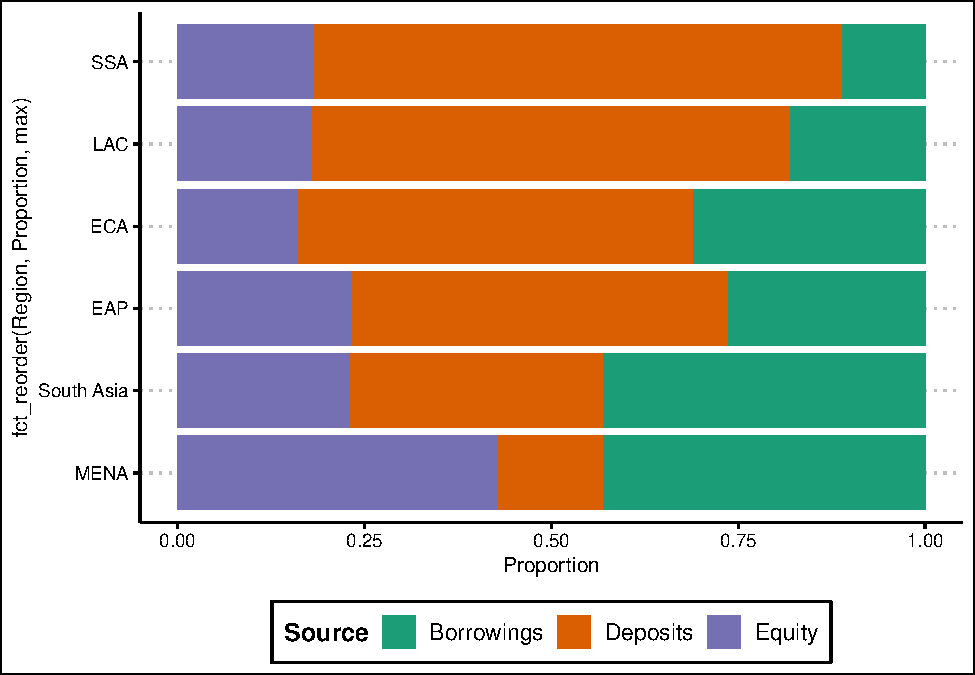
\includegraphics{02-rmd-basics-markdown_files/figure-latex/unnamed-chunk-5-1.pdf}
\caption{\label{fig:unnamed-chunk-5}Funding structure of MFIs Across the Globe by Region (2015)}
\end{figure}

Although the transformation of NGOs has its merits, most MFIs have still not transformed\autocite{d2017ngos}. Therefore, a key output of the proposed study will be the motives behind some MFIs transforming while other MFIs retain the NGO model. The current literature has been overly concerned with the transformed MFIs and not addressed this issue. Even among the transformed MFIs, researchers have not uncovered the drivers of the decision by MFIs to transform and the necessary preconditions for transformation. The existing research takes for granted that MFIs transform to be sustainable. Given the benefits of transformation touted in the numerous studies, then most MFIs should have already transformed.

Moreover, as \textcite{morduch2019challenges} argues, if there is no trade-off between financial performance and social performance of transformed MFIs, then NGOs would not exist. However, this is not the case. It appears, therefore that some additional factors influence the decision by MFI to either transform or retain the NGO model. As noted, there is no conclusive evidence on the effects of MFI transformation on their performance. These contradicting results could be because of numerous unknown reasons. It is in order, therefore, to establish the factors that influence the sustainability and outreach of transformed MFIs. Similarly, establishing the factors that moderate the relationship between capital structure on the one hand and the financial performance and social performance of MFIs in Africa will be a novel contribution to the research.

Recent literature also suggests that the performance of MFIs is dependent on the broader macroeconomic conditions as well \textcite{ahlin2011does}, and is country-specific \autocite{d2017ngos}. Thus, in the analysis of the institutional transformation of MFIs, cross-country and regional differences must be factored in. However, most studies have not considered the cross country and regional variations. Failure to consider regional disparities means that the extant research fails to capture local contextual peculiarities.

These regional differences motivate the choice of MFIs in Africa as the unit of analysis. By focusing on Africa, the study will isolate the regional and country heterogeneity of the effects of transformation, an issue that could have affected the results of research based on pooled global datasets. Thus, the output of the study will be unique to Africa and therefore more actionable. To sum up this section, the proposed study significantly extends the existing literature on MFI transformation. The next section outlines the purpose statement.

\hypertarget{purpose-statement}{%
\section{Purpose Statement}\label{purpose-statement}}

\noindent The primary aim of this proposed research is to evaluate how the the transformation of MFIs in Africa impacts their financial and social performance.

\hypertarget{research-questions}{%
\section{Research Questions}\label{research-questions}}

\noindent The study specifically seeks answers to the following research questions.

\begin{enumerate}
\def\labelenumi{\arabic{enumi}.}
\tightlist
\item
  Why do some MFIs in Africa transform into the commercial model while others retain the NGO Model?
\item
  To what extent has the institutional transformation of MFIs in Africa affected financial inclusion?
\item
  After transformation, what factors explain the joint level of sustainability and outreach by MFIs in Africa?
\item
  What are the factors that influence the choice of financing sources by transformed MFIs in Africa?
\item
  How is capital structure related to the performance of transformed MFIs in Africa?
\end{enumerate}

\hypertarget{significance-of-the-study}{%
\section{Significance of the Study}\label{significance-of-the-study}}

\noindent In pursuing the stated objectives, this study will fill a theoretical deficiency in the capital structure of quasi-commercial organisations that have a social dimension of value. The context of shareholder and debtholder primacy was the foundation of the development of capital structure theories. Arguments from this genesis of capital structure theories have failed to factor in corporations with extra dimensions of value, such as the achievement of social goals. As a case in point, \texttt{Modigliani\ and\ Miller} capital structure theory may not be entirely applicable to MFIs where value also has a social facet. In the Modigliani and Miller capital structure theory, the value of a firm is the sum of equity and debt components in the capital structure of a corporation. The value of a company is an increasing function of the debt proportion of capital structure up to the point where the costs of financial distress outweigh the benefits of the interest tax shield.In the process, the study will also fill an empirical deficit on the relationships between capital structure on the one hand, and financial performance, social performance, and efficiency of transformed MFIs in Africa. The empirical output has implications on policy direction relating to MFIs in Africa.

The study also has a variety of policy implications. These policy implications are related to the research objectives. For instance, what are the factors that drive MFIs to transform or fail to transform? The answer to this question would inform the crafting of policy if transformation is indeed desirable. Moreover, what are the drivers of financial inclusion, outreach, and sustainability of MFIs after the transformation? Lastly, what are the determinants of the choice of financing sources? It is worth noting that if the drive for institutional transformation is to achieve the desired effects, then the change in the MFI funding structures must not compromise the achievement of social objectives. If the conversion of MFIs negatively affects social performance, there would be no way to justify the transformation of MFIs. If indeed the transformation of MFIs was meant to improve their sustainability, this must not be to the detriment of social performance.

Also, if the transition results a decline in social performance, then the transformation could be treated as the transition point of transformed MFIs into the mainstream banking system \autocite{kent2013bankers}. It is crucial therefore to investigate the outcomes of the change to inform the design of a framework that would not expose the poor and financially excluded to the same level of exclusion by the financial system that MFIs ought to address. Doing this would be tantamount to allowing MFIs to use the underprivileged as a ladder to climb into the mainstream system, and abandoning them shortly after, which raises ethical questions.

Similarly, the identification of factors that influence the choice of financing structures has implications for the design of policies aimed at the capital market. For the same reasons, the identification of factors that influence the social performance of transformed MFIs will also be useful, not just for policy design, but also for managerial decision making. Also, the calibration of a mix of debt and equity for transformed MFIs that optimises financial and social performance will inform both policy-making and managerial decision making.

Finally, the efficiency of MFIs is a significant determinant of both the financial and social performance of MFIs. According to the efficiency theory, the positive relationship between concentration and profitability is indicative of the tendency of firms that are efficient to be successful and hence dominant in their industries \autocite{lipczynski2005industrial}. Efficiency gains could result from economies of scale and cost-saving schemes initiated by the management. Enhanced efficiency by MFIs is, therefore desirable. However, the efficiency of MFIs should encompass both financial and social dimensions. The entry of commercial sources of capital may affect the both the financial and social efficiency of MFIs in line with agency theory. It is therefore vital to establish the relationship between capital structure and efficiency to inform both the management and stakeholders of the dynamics in the MFI sector regarding effectiveness in the new era of commercial funding.

\hypertarget{outline-of-the-study}{%
\section{Outline of the Study}\label{outline-of-the-study}}

\noindent The remainder of the study will be structured as follows. Chapter two locates microfinance in the financial intermediation space and traces the genesis and evolution of the transformation. Chapter three lays out the theoretical framework of the study, focusing on the agency theory and profit incentives, capital structure theory, and the institutional theory. The subsequent five chapters each delves into one research question, laying out the methodologies applied and the results. The last chapter concludes.


%%%%% REFERENCES

% JEM: Quote for the top of references (just like a chapter quote if you're using them).  Comment to skip.
% \begin{savequote}[8cm]
% The first kind of intellectual and artistic personality belongs to the hedgehogs, the second to the foxes \dots
%   \qauthor{--- Sir Isaiah Berlin \cite{berlin_hedgehog_2013}}
% \end{savequote}

\setlength{\baselineskip}{0pt} % JEM: Single-space References

{\renewcommand*\MakeUppercase[1]{#1}%
\printbibliography[heading=bibintoc,title={\bibtitle}]}

\end{document}
